\section{RVV}\label{chap:bg:sec:rvv}
% RISC-V has extensions
RISC-V is an open family of ISAs which defines ``base integer ISAs'' (e.g. all 64-bit RISC-V cores implement the RV64I Base Integer Instruction Set) and extensions (e.g. the ``M'' extension for integer multiplication).
A base instruction set combined with a set of extensions (\todomark{example of a architecture/feature string}) is known as a RISC-V ISA.
Because RISC-V is open, anyone can design, manufacture, and sell chips implementing any RISC-V ISA.
% RVV is the vector one
RVV is the officially ratified vector extension for RISC-V, and going forward all RISC-V chips with vector processing capabilities should implement it instead of designing their own custom vector extensions.
This section summarizes Sections 1-9 and 17 of the RVV Specification v1.0\cite{RISCVVectorExtension2021}.

%---------------------------------
%---------------------------------
%---------------------------------
\subsection{Vector model}\label{chap:bg:sec:rvv:vector_model}
\emph{Summarizes \cite[Sections 1-4]{RISCVVectorExtension2021}}
\todomark{Add prestart/active/inactive/body/tail definitions, would bump up to 1-5}


\figinput[width=0.7\textwidth,pos=h]{1_20Background/figures/fig_RVV_simple_widths}
\figinput[width=0.7\textwidth,pos=h]{1_20Background/figures/fig_RVV_added_state}


RVV defines thirty-two vector registers, each of an implementation-defined width VLEN.
These registers can be interpreted as \emph{vectors} of \emph{elements}.
The program can configure the size of elements, and the implementation defines a maximum width ELEN.
\cref{fig:RVV_simple_widths} shows a simple example of a 128-bit vector, where the maximum element length is 32-bits.


RVV also adds some state that defines how the vector registers are used (see \cref{fig:RVV_added_state}).
These are stored in RISC-V Control and Status Registers (CSRs), which the program can read.

%---------------------------------
\subsubsection{\code{vl} and \code{vstart}}\label{chap:bg:sec:rvv:vstart}
The first CSR is the Vector Length \code{vl}, which holds the number of elements that could be updated from a vector instruction.
The program updates this value through fault-only-first loads (\cref{chap:bg:sec:rvv:fof}) and more commonly the \code{vsetvl} instruction family (\cref{chap:bg:sec:rvv:vsetvl}).

In the simple case, \code{vl} is equal to the total available elements (see \cref{fig:RVV_vl_full}).
It can also be fewer (see \cref{fig:RVV_vl_short}), in which case vector instructions will not write to elements in the \enquote{tail} (i.e. elements past \code{vl}).
This eliminates the need for a `cleanup loop' common in fixed-length vector programs.

\figinput[width=0.7\textwidth,pos=t]{1_20Background/figures/fig_RVV_vl}

In a similar vein, \code{vstart} specifies \enquote{the index of the first element to be executed by a vector instruction}.
This is usually only set by the hardware whenever it is interrupted mid-instruction (see \cref{fig:RVV_vstart_trap}) so that the instruction can be re-executed later without corrupting completed values.
Whenever a vector instruction completes, \code{vstart} is reset to zero.

The program \emph{can} set \code{vstart} manually, but it may not always work.
If an implementation couldn't arrive at the value itself, then it is allowed to reject it.
The specification gives an example where a vector implementation never takes interrupts during an arithmetic instruction, so it would never set \code{vstart} during an arithmetic instruction, so it could raise an exception if \code{vstart} was nonzero for an arithmetic instruction.

\figinput[width=0.7\textwidth,pos=t]{1_20Background/figures/fig_RVV_vstart_trap}

%---------------------------------
\subsubsection{\code{vtype}}
\code{vtype} contains two key fields that describe how vector instructions interpret the contents of vector registers.
The first is the Selected Element Width (\code{SEW}), which is self-explanatory.
It can be 8, 16, 32, or 64.
128-bit elements are referenced a few times throughout but haven't been formally specified (see \cite[p32]{RISCVVectorExtension2021}).
Most instructions\footnote{Except where the width is encoded in the instruction, like bytemask loads.} will split vector registers into elements of this width.

The second field is the Vector Register Group Multiplier (\code{LMUL}).
Vector instructions don't just operate over a single register, but over a register \emph{group} as defined by this field.
For example, if \code{LMUL=8} then each instruction would operate over 8 register's worth of elements.
These groups must use aligned register indices, so if \code{LMUL=4} all vector register operands should be multiples of 4 e.g. \code{v0, v4, v8} etc.
In some implementations this may increase throughput, which by itself is beneficial for applications.

\figinput[width=0.7\textwidth,pos=t]{1_20Background/figures/fig_RVV_LMUL_widening}

However, the true utility of \code{LMUL} lies in widening/narrowing operations (see \cref{fig:RVV_LMUL_widening}).
For example, an 8-by-8-bit multiplication can produce 16-bit results.
Because the element size doubles, the number of vector registers required to hold the same number of elements also doubles.
Doubling \code{LMUL} after such an operation allows subsequent instructions to handle all the results at once.
At the start of such an operation, fractional \code{LMUL} (1/2, 1/4, or 1/8) can be used to avoid subsequent results using too many registers.
% high register usage in subsequent operations.
% If such operations end up using too many registers, fractional LMUL (1/2, 1/4, or 1/8) can be used to 

\code{vtype} also encodes two flags: mask-agnostic and tail-agnostic.
If these are set, the implementation is \emph{allowed} to overwrite any masked-out or tail elements with all 1s.

Most vector instructions will interpret their operands using \code{vtype}, but this is not always the case.
Some instructions (such as memory accesses) use different Effective Element Widths (\code{EEW}) and Effective LMULs (\code{EMUL}) for their operands.
In the case of memory accesses, the \code{EEW} is encoded in the instruction bits and the \code{EMUL} is calculated to keep the number of elements consistent.
Another example is widening/narrowing operations, which by definition have to interpret the destination registers differently from the sources.

\pagebreak
\figinput[width=0.8\textwidth,pos=h]{1_20Background/figures/fig_RVV_mask_example}
%---------------------------------
\subsubsection{Masking}\label{chap:bg:sec:rvv:masking}
Most vector instructions allow for per-element \emph{masking} (see \cref{fig:RVV_mask_example}).
When masking is enabled, register \code{v0} acts as the `mask register', where each bit corresponds to an element in the vector.
If the mask bit is 0, that element is \emph{active} and will be used as normal.
If the mask bit is 1, that element will be \emph{inactive} and not written to (or depending on the mask-agnostic setting, overwritten with 1s).
When masking is disabled, all elements are \emph{active}.

\todomark{There will always be enough bits in a single register to mask all elements. maximum element count comes from smallest SEW (8 bits) and largest LMUL (8 registers). Max elements = VLEN * LMUL / SEW = VLEN * 8 / 8 = VLEN elements, there are VLEN bits in a single register.}

\figinput[width=0.8\textwidth,pos=h]{1_20Background/figures/fig_RVV_examples_combined}
%---------------------------------
\subsubsection{Summary}
\cref{fig:RVV_examples_combined} shows all of the above features used in a single configuration:
\begin{itemize}
    \item The instruction was previously interrupted and restarted, so \code{vstart=2}
    \item Elements are 16-bit
    \item \code{LMUL=4} to try and increase throughput
    \item Only 29 of the 32 available elements were requested, so \code{vl=29} (3 tail elements)
    \item Some elements are masked out/inactive (in this case seemingly at random)
    \item Overall, 21 elements are active
\end{itemize}

\pagebreak
%---------------------------------
%---------------------------------
%---------------------------------
\subsection{Strip mining and \code{vsetvl}}\label{chap:bg:sec:rvv:vsetvl}
\emph{Summarizes \cite[Section 6]{RISCVVectorExtension2021}}
\todomark{This section would introduce the general programming paradigm for scalable vectors and the \code{vsetvl} instruction family.
\code{vsetvl} instructions just set \code{vtype}, so in the interests of word count maybe this isn't necessary?}

\pagebreak
%---------------------------------
%---------------------------------
%---------------------------------
\subsection{Exception handling}
\emph{Summarizes \cite[Section 17]{RISCVVectorExtension2021}}

During the execution of a vector instruction, two events can prevent an instruction from fully completing: a synchronous exception in the instruction itself, or an asynchronous interrupt from another part of the system.
Implementations may choose to wait until an instruction fully completes before handling asynchronous interrupts, making it unnecessary to pause the instruction halfway through, but synchronous exceptions cannot be avoided in this way (particularly for those performing memory accesses).

The RVV specification defines two modes for `trapping' these events, which implementations may choose between depending on the context (e.g. the offending instruction), and notes two further modes which may be used in further extensions.
All modes start by saving the PC of the trapping instruction to a CSR \code{*epc}.

%---------------------------------
\subsubsection{Imprecise vector traps}
Imprecise traps are intended for events that are not recoverable, where \enquote{reporting an error and terminating execution is the appropriate response}.
They do not impose any extra requirements on the implementation.
For example, an implementation that executes instructions out-of-order does not need to guarantee that instructions older than \code{*epc} have completed, and is allowed to have completed instructions newer than \code{*epc}.

If the trap was triggered by a synchronous exception, the \code{vstart} CSR must be updated with the element that caused it.
\todomark{inconsistency in spec - Ch17 first para says "the vstart CSR contains the element index on which the trap was taken", but the imprecise trap section only specifies this for synchronous exceptions}

The specification also states \enquote{There is no support for imprecise traps in the current standard extensions}, \todomark{what does this mean?}

%---------------------------------
\subsubsection{Precise vector traps}
Precise vector traps are intended for instructions that can be resumed after handling the interrupting event.
This means the architectural state (i.e. register values) when starting the trap could be saved and reloaded before continuing execution.
Therefore it must look like instructions were completed in-order, even if the implementation is out-of-order:
\begin{itemize}
    \item Instructions older than \code{*epc} must have completed (committed all results to the architectural state)
    \item Instructions newer than \code{*epc} must \textbf{not} have altered architectural state.
\end{itemize}

On a precise trap, regardless of what caused it, the \code{vstart} CSR must be set to the element index on which the trap was taken.
The save-and-reload expectation then add two constraints on the trapping instruction's execution:
\begin{itemize}
    \item Operations affecting elements preceding \code{vstart} must have committed their results
    \item Operations affecting elements at or following \code{vstart} must either
    \begin{itemize}
        \item not have committed results or otherwise affected architectural state
        \item be \emph{idempotent} i.e. produce exactly the same result when repeated.
    \end{itemize}
\end{itemize}

The idempotency option gives implementations a lot of leeway.
Some instructions \todomark{examples} are specifically prohibited from overwriting their inputs to make them idempotent.
If an instruction is idempotent, an implementation is even allowed to repeat operations on elements \emph{preceding} \code{vstart}.
However for memory accesses the idempotency depends on the memory being accessed.
For example, writing to a memory-mapped I/O region may not be idempotent.

Another memory-specific issue is that of \emph{demand-paging}, where the OS needs to step in and move virtual memory pages into physical memory for an instruction to use.
This use-case is specifically called out by the specification for precise traps.
Usually, this is triggered by some element of a vector memory access raising a synchronous exception, invoking a precise trap, and \todomark{using \code{vstart} to show the OS which address it wants?}
Because \code{vstart} must be set to the element that demanded the page, and operations preceding \code{vstart} must have completed, any elements that could potentially trigger demand-paging \emph{must} wait for the preceding elements to complete.
This always applies, no matter what the instruction's specific ordering guarantees are.

%---------------------------------
\subsubsection{Other modes}
The RVV spec mentions two other potential trap modes.
First is \enquote{Selectable precise/imprecise traps}, where an implementation provides a bit that selects between precise or imprecise traps.
The intent is to allow precise traps to be selected for e.g. debugging purposes, and for imprecise traps to be selected for extra performance.

The second mode is \enquote{Swappable traps}, where a trap handler could use special instructions to \enquote{save and restore the vector unit microarchitectural state}.
The intent seems to be to support context switching with imprecise traps, which could also require the \emph{opaque} state (i.e. internal state not visible to the program) to be saved and restored.
Right now, it seems that context switching always requires a precise trap.

Neither of these modes are actually defined, but they are simply noted as possibilities for the future.

\pagebreak
%---------------------------------
%---------------------------------
%---------------------------------
\subsection{Memory access instructions}
\emph{Summarizes \cite[Sections 7-9]{RISCVVectorExtension2021}}

RVV defines five broad categories of memory access instructions, which this subsection describes.
For the most part, they handle their operands as described in \cref{chap:bg:sec:rvv:vector_model}.
\code{EEW} and \code{EMUL} are usually derived from the instruction encoding, rather than reading the \code{vtype} CSR.
In a few cases the Effective Vector Length \code{EVL} is different from the \code{vl} CSR, so for simplicity all instructions are described in terms of \code{EVL}.

\subsubsection{Segment accesses}
Three of the five categories (unit/strided, fault-only-first, and indexed) support \emph{segmented} access.
This is used for unpacking contiguous structures of $n$ \emph{fields} and placing each field in a separate vector.
\cref{fig:RVV_mem_unit} demonstrates a common example: the extraction of separate R, G, and B components from a color.
Without segmentation, i.e. $n = 1$, each consecutive memory address maps to a consecutive element in a single vector register group.
With segmentation, elements are grouped into segments of $n > 1$ fields, where each field is mapped to a different vector register group.
This principle extends to \code{LMUL > 1} (\cref{fig:RVV_mem_lmul_3seg}).

\todomark{vl, vstart, masks are all in terms of segments in segmented accesses.}
\todomark{if a trap occurs, it is implementation defined if a subset of the faulting segment's accesses are performed before the trap is taken}
\todomark{nf has range 1..8}

\figinput[width=0.48\textwidth,pos=h]{1_20Background/figures/fig_RVV_mem_unit}
\figinput[width=0.55\textwidth,pos=h]{1_20Background/figures/fig_RVV_mem_lmul_3seg}

\newcommand{\param}[1]{\textbf{\textcolor{Blue}{#1}}}
\newcommand{\paramt}[1]{\code{\param{#1}}}


\pagebreak
%%%%%%%%%%%%%%%%%%%%%%%%%%%%%%%%%%%%%%%%%%
\subsubsection{Unit and Strided accesses}\label{chap:bg:sec:rvv:unitstrideaccess}

\begin{figure}[h]
    \centering
    \begin{subfigure}{\textwidth}
        \centering
        \large (Unit) \code{vlseg\param{<nf>}e\param{<eew>}.v vd, (rs1), vm} \\
(Strided) \code{vlsseg\param{<nf>}e\param{<eew>}.v vd, (rs1), rs2, vm}
        \caption{Instruction}
    \end{subfigure}
    \vspace{1em}
    
    \begin{subtable}[b]{0.5\textwidth}
    \begin{tabular}{ll}
    \toprule
    Masked? & \code{vm == 0} \\
        \code{stride} & (Unit) \code{\param{<eew>} * \param{<nf>}} \\
                    & (Strided) From \code{rs2} \\
        \code{EEW} & \paramt{<eew>} \\
        \code{EVL} & \code{vl} \\
        \code{EMUL} & \code{VLEN * \param{<eew>} / EVL} \\
        \code{NFIELDS} & \paramt{<nf>} \\
        \bottomrule
    \end{tabular}
    \caption{How fields are interpreted}
    \label{tab:RVV_mem_strided}
    \end{subtable}\hfill
    \begin{subfigure}[b]{0.5\textwidth}
        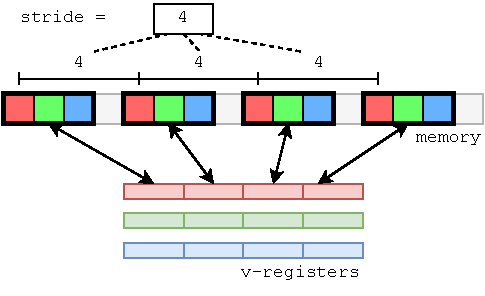
\includegraphics[width=\textwidth]{Figures/RVV_mem_strided_3seg.pdf}
        \caption{Example of a segmented strided access\\\code{EEW=8-bits}, \code{nf=3}, \code{stride=4},\code{EVL=4}}
        \label{fig:RVV_mem_strided_3seg}
    \end{subfigure}
    \caption{Segmented Unit/Strided Access Information}
\end{figure}

\noindent
Moves active elements of \paramt{nf} vector register groups to/from contiguous segments of memory,
where each segment is separated by \code{stride} bytes.

\begin{itemize}
    \item The start of each segment is separated by \code{stride} bytes.
    \begin{itemize}
        \item The Unit version (short for Unit-stride) tightly packs segments, equivalent to selecting \code{stride = \param{nf} * \param{eew} / 8}.
        \item \code{stride} may be negative or zero.
        \item If \code{rs2} is register \code{x0}, implementations may perform fewer than \code{EVL} memory accesses. Otherwise, they must appear to perform all memory accesses, even if the value of \code{rs2} is zero.
    \end{itemize}
    % These two are described by the diagram
    % \item Each segment is \code{\param{nf} * \param{eew}} bits long, i.e. \paramt{nf} elements long.
    % \item Each element in the $i$-th segment maps to the $i$-th element of a vector register group.
    \item This instruction doesn't do anything if the \code{vstart >= EVL}.
\end{itemize}


% ORDERING
\noindent
\emph{Ordering}
\\\noindent
There are no ordering guarantees, other than those required by precise vector traps (if used).



% EXCEPTION HANDLING
\noindent
\emph{Exception Handling}
\\\noindent
If any element within segment $i$ triggers a synchronous exception, \code{vstart} is set to $i$ and a precise or imprecise trap is triggered.
Load instructions may overwrite active segments past the segment index at which the trap is reported, but not past \code{EVL}.\cite[Section 7.7]{RISCVVectorExtension2021}
Upon entering a trap, it is implementation-defined how much of the faulting segment's accesses are performed.

% Unit accesses, where segments are tightly packed, can be expressed in terms of strided accesses where segments can have arbitrary separation.
% \todomark{negative strides supported}

% \todomark{Load instructions may overwrite active destination vector register group elements past the element index at which the trap is
% reported.}\cite[Section 7.7]{RISCVVectorExtension2021}

\subsubsection{Unit fault-only-first loads}\label{chap:bg:sec:rvv:fof}


\begin{table}[h]
    \centering
    % \begin{subfigure}[b]{0.5\textwidth}
    %     \centering
    %     \caption{Instruction}
    % \end{subfigure}\hfill
    % \begin{subtable}[b]{0.5\textwidth}
    \centering
\begin{tabular}{ll}
\multicolumn{2}{c}{\large \code{vlseg\param{<nf>}e\param{<eew>}ff.v vd, (rs1), vm}} \\
    \toprule
    Masked? & \code{vm == 0} \\
        \code{EEW} & \paramt{<eew>} \\
        \code{EVL} & \code{vl} \\
        \code{EMUL} &  \code{VLEN * \param{<eew>} / EVL} \\
        \code{NFIELDS} & \paramt{<nf>} \\
    \bottomrule
\end{tabular}
    \caption{Unit Fault-only-First Information}
    \label{tab:RVV_mem_fof}
    % \end{subtable}\hfill
\end{table}

This is equivalent to a unit load in all respects but exception handling.
If any access in segment 0 raises an exception\footnote{Segment 0 may be masked out, in which case this is impossible.}, \code{vl} is not modified and the trap is taken as usual.
If any access in any active segment $> 0$ raises an exception, the trap is not taken, \code{vl} is reduced to the index of the offending segment, and the instruction finishes.
If an asynchronous interrupt is encountered at any point, the trap is taken and \code{vstart} is set as usual.

Similar to plain loads, if an exception is encountered the instruction is allowed to update segments past the offender (but not past the original \code{vl}).
If any synchronous exception or asynchronous interrupt occurs, regardless of the segment index, it is implementation-defined how much of the faulting segment's accesses are performed.

\pagebreak
%%%%%%%%%%%%%%%%%%%%%%%%%%%%%%%%%%%%%%%%%%
\subsubsection{Indexed accesses}
\begin{figure}[h]
    \centering
    \begin{subfigure}{\textwidth}
        \centering
        \large \code{vl\param{<u|o>}xseg\param{<nf>}e\param{<eew>}.v vd, (rs1), vs2, vm}
        \caption{Instruction}
    \end{subfigure}
    \vspace{1em}
    
    \begin{subtable}[b]{0.5\textwidth}
    \begin{tabular}{ll}
    \toprule
        Masked? & \code{vm == 0} \\
    \midrule
        Element \code{EEW} & \code{vtype.SEW} \\
        Element \code{EMUL} & \code{vtype.LMUL} \\
        \midrule
        Ordered? & \paramt{<u|o>} \\
        Index Vector & \code{vs2} \\
        Index \code{EEW} & \paramt{<eew>} \\
        Index \code{EMUL} & \code{VLEN * \param{<eew>} / EVL} \\
        \midrule
        \code{NFIELDS} & \paramt{<nf>} \\
        \code{EVL} & \code{vl} \\
        \bottomrule
    \end{tabular}
    \caption{How fields are interpreted}
    \label{tab:RVV_mem_index}
    \end{subtable}\hfill
    \begin{subfigure}[b]{0.5\textwidth}
        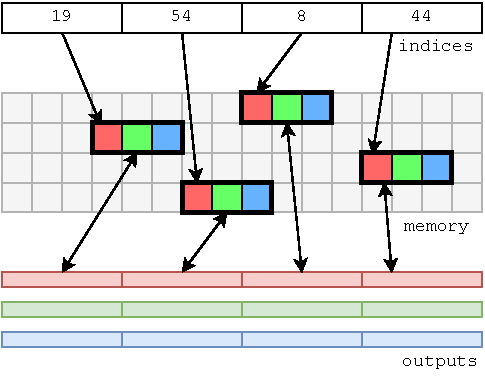
\includegraphics[width=\textwidth]{Figures/RVV_mem_index_3seg.pdf}
        \caption{Example of a segmented indexed access\\\code{EEW=8-bits}, \code{nf=3}}
        \label{fig:RVV_mem_index_3seg}
    \end{subfigure}
    \caption{Segmented Indexed Access Information}
\end{figure}

% As for unit/strided, this instruction moves elements from \paramt{nf} register groups to/from contiguous segments of memory.
% The segment locations are generated from a vector of byte-address offsets\footnote{The term `index' can be misleading. In other scenarios, such as C, `indexing' an array specifies an index in units of elements. This is not the case here.}.
% The start of segment $i$ is the base address offset by \code{offset_vector[i]}.

Moves elements of \paramt{nf} vector register groups to/from contiguous segments of memory,
where each segment is offset by an index (in bytes) taken from another vector.

\begin{itemize}
\item The start of each segment is defined by \code{base address + index\_vector[i]}.
% \item Each segment is \paramnf * eew` bits long, i.e. [nf] elements long.
% \item Each element in the i-th segment maps to the i-th element of a vector register group.
% \item Accesses within each segment are not ordered relative to each other.
% \item If the ordered variant of this instruction is used, then the segments must be accessed in the order specified by the index vector.
\item This instruction doesn't do anything if \code{vstart >= EVL}.
\end{itemize}

% ORDERING
\noindent
\emph{Ordering}
\\\noindent
Accesses within each segment are not ordered relative to each other.
If the ordered variant of this instruction is used, then the segments must be accessed in order (i.e. 19, 54, 8, 44 for \cref{fig:RVV_mem_index_3seg}).
Otherwise, segment ordering is not guaranteed.


% EXCEPTION HANDLING
\noindent
\emph{Exception Handling}
\\\noindent
If any element within segment $i$ triggers a synchronous exception, \code{vstart} is set to $i$ and a precise or imprecise trap is triggered.
Load instructions may overwrite active segments past the segment index at which the trap is reported, but not past \code{EVL}\cite[Section 7.7]{RISCVVectorExtension2021}.
Upon entering a trap, it is implementation-defined how much of the faulting segment's accesses are performed.
% \todomark{for implementations with precise vector traps, exceptions on indexed-unordered stores must also be precise}\cite[p30]{RISCVVectorExtension2021}
% \todomark{Load instructions may overwrite active destination vector register group elements past the element index at which the trap is
% reported.}\cite[Section 7.7]{RISCVVectorExtension2021}

\pagebreak
\subsubsection{Unit whole-register accesses}
% \begin{tabular}{ll}
% \toprule
%     \code{EEW} & From Instruction \\
%     \midrule
%     \code{NFIELDS} & From Instruction \\
%     \code{EVL} & \code{NFIELDS * VLEN / EEW} \\
%     \bottomrule
% \end{tabular}
\begin{table}[h]
    \centering
    % \begin{subfigure}[b]{0.5\textwidth}
    %     \centering
        % \large \code{vl\param{<nreg>}re\param{<eew>}.v vd, (rs1)}
    %     \caption{Instruction}
    % \end{subfigure}\hfill
    % \begin{subtable}[b]{0.5\textwidth}
    % \centering
\begin{tabular}{ll}
    \multicolumn{2}{c}{\large \code{vl\param{<nreg>}re\param{<eew>}.v vd, (rs1)}} \\
\toprule
        Masked? & False \\
        Number of Registers & \paramt{<nreg>} \\
        \code{EEW} & \paramt{<eew>} \\
        \code{EVL} & \code{NFIELDS * VLEN / EEW} \\
        \code{EMUL} & 1 \\
    \bottomrule
\end{tabular}
    \caption{Unit Whole Register Information}
    \label{tab:RVV_mem_wholereg}
    % \end{subtable}\hfill
\end{table}

Moves the contents of \paramt{nreg} vector registers to/from a contiguous range in memory.
Equivalent to a unit-stride access where \code{EVL} equals the total number of elements in \paramt{nreg} registers.
\begin{itemize}
    \item \code{nreg} must be a power of two.
    \item Doesn't support segmented access.
    \item This instruction doesn't do anything if \code{vstart >= EVL}.
\end{itemize}

Ordering and exception handling are identical to unit-stride accesses (\cref{chap:bg:sec:rvv:unitstrideaccess}).
% \todomark{ordering}
% \todomark{Exceptions}

\subsubsection{Unit bytemask accesses}
% \begin{tabular}{ll}
% \toprule
%     \code{EEW} & 8-bits \\
%     \code{EMUL} & 1 \\
%     \midrule
%     \code{EVL} & \code{ceil(vl/8)} \\
%     \bottomrule
% \end{tabular}
\begin{table}[h]
    \centering
    % \begin{subfigure}[b]{0.5\textwidth}
    %     \centering
    %     \large \code{vlm.v vd, (rs1)}
    %     \caption{Instruction}
    % \end{subfigure}\hfill
    % \begin{subtable}[b]{0.5\textwidth}
\begin{tabular}{ll}
\multicolumn{2}{c}{\large \code{vlm.v vd, (rs1)}} \\
    \toprule
        Masked? & False \\
        \code{EEW} & 8-bits \\
        \code{EVL} & \code{ceil(vl/8)} \\
        \code{EMUL} & 1 \\
    \bottomrule
\end{tabular}
    \caption{Unit Bytemask Information}
    \label{tab:RVV_mem_bytemask}
    % \end{subtable}\hfill
\end{table}

Moves the contents of a mask register to/from a contiguous range of memory.
This instruction transfers at least \code{vl} bits,
one bit for each element that could be used in subsequent vector instructions.
This will always fit in a single vector register (see \cref{chap:bg:sec:rvv:masking}), hence \code{EMUL = 1} in all cases.
\begin{itemize}
    \item This instruction always operates as if the tail-agnostic setting of \code{vtype} is true.
    \item This instruction doesn't support segmented access.
    \item This instruction doesn't do anything if \code{vstart >= EVL}.
\end{itemize}
Ordering and exception handling are identical to unit-stride accesses (\cref{chap:bg:sec:rvv:unitstrideaccess}).

\pagebreak
%---------------------------------
%---------------------------------
%---------------------------------
\subsection{Implementations}
\todomark{Planned to do a survey of existing implementations here - might be too many words?}